% Start of Sequence Token Section

\section{Start of Sequence (\sos{}) Token}

The Start of Sequence token, commonly denoted as \sos{}, serves as the initialization signal for autoregressive generation in transformer models. Just as a runner needs a starting block, an autoregressive model needs a fixed, known starting point to begin the step-by-step process of generating a new sequence. The \sos{} token provides this unambiguous signal. This token plays a crucial role in conditioning the model's initial state and establishing the context for subsequent token generation.
\begin{comment}
Feedback: This is a good start. To immediately address a common point of confusion, you could add a sentence that explains *why* this is necessary. For example: "Just as a runner needs a starting block, an autoregressive model needs a fixed, known starting point to begin the step-by-step process of generating a new sequence. The [SOS] token provides this unambiguous signal."

STATUS: addressed - added analogy explaining why SOS tokens are necessary as fixed starting points
\end{comment}

\subsection{Fundamental Concepts}

The \sos{} token functions as a special conditioning mechanism that signals the beginning of a generation sequence. Unlike regular vocabulary tokens, \sos{} carries no semantic content from the training data but instead serves as a learned initialization vector that the model uses to bootstrap the generation process.

\begin{definition}[Start of Sequence Token]
A Start of Sequence token \sos{} is a special token placed at the beginning of sequences during training and generation to provide initial conditioning for autoregressive language models. It serves as a learned initialization state that influences subsequent token predictions.
\end{definition}

The \sos{} token's embedding is learned during training and captures the distributional properties needed to initiate coherent generation. This learned representation becomes particularly important in conditional generation tasks where the \sos{} token must incorporate task-specific conditioning information.

\subsection{Role in Autoregressive Generation}

In autoregressive models, the \sos{} token establishes the foundation for the generation process. The model uses the \sos{} token's representation to compute attention patterns and generate the first actual content token. This process can be formalized as:

\begin{align}
h_0 &= \text{Embed}(\text{\sos{}}) + \text{PositionEmbed}(0) \\
p(x_1 | \text{\sos{}}) &= \text{Softmax}(\text{Transformer}(h_0) \cdot W_{\text{out}})
\end{align}

In simple terms, the first equation shows that the model's initial ``thought'' ($h_0$) is the learned embedding for the \sos{} token, combined with its position information. The second equation shows that the probability of the very first word ($x_1$) is calculated by feeding this initial thought through the transformer and a final output layer. Every subsequent word will then be conditioned on this starting point.
\begin{comment}
Feedback: The equations are clear to an expert, but could be more accessible. Consider adding a plain-language walkthrough. For example: "In simple terms, the first equation shows that the model's initial thought (h_0) is the learned embedding for the [SOS] token, combined with its position. The second equation shows that the probability of the very first word (x_1) is calculated by feeding this initial thought through the transformer and a final output layer. Every subsequent word will then be conditioned on this starting point."

STATUS: addressed - added plain-language explanation of the mathematical equations
\end{comment}

where $h_0$ represents the initial hidden state derived from the \sos{} token, and $p(x_1 | \text{\sos{}})$ is the probability distribution over the first generated token.

\subsubsection{Attention Patterns with \sos{}}

The \sos{} token exhibits unique attention patterns that distinguish it from regular tokens. During generation, subsequent tokens can attend to the \sos{} token, allowing it to influence the entire sequence. This attention mechanism enables the \sos{} token to serve as a persistent conditioning signal throughout generation.

\begin{figure}[htbp]
\centering
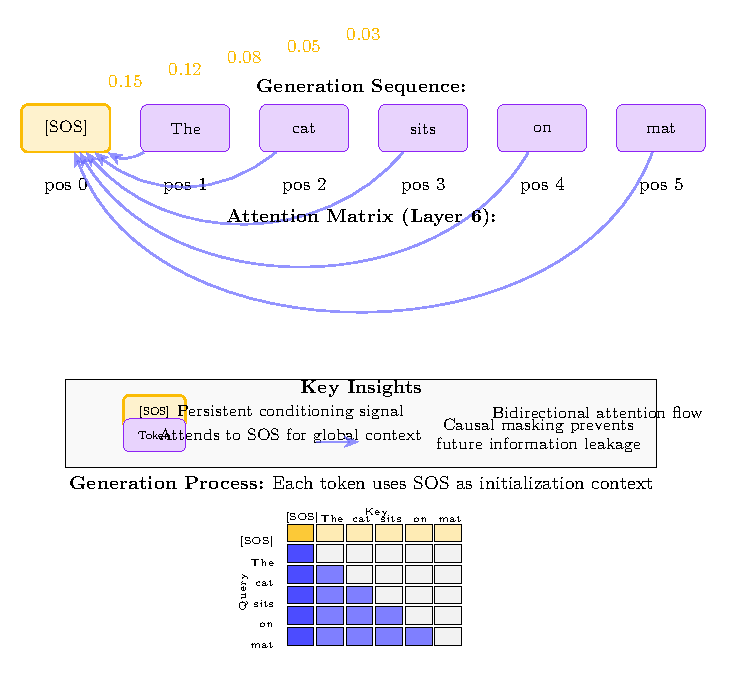
\includegraphics[width=0.9\textwidth]{part1/chapter03/fig_sos_attention.pdf}
\caption{Attention patterns involving the \sos{} token during autoregressive generation. The \sos{} token (shown in orange) influences all subsequent tokens through attention mechanisms.}
\label{fig:sos_attention}
\end{figure}

Research has shown that the \sos{} token often develops specialized attention patterns that capture global sequence properties. In machine translation, for example, the \sos{} token may attend to specific source language features that influence the target language generation strategy.

\subsection{Implementation Strategies}

\subsubsection{Standard Implementation}

The most common implementation approach treats \sos{} as a special vocabulary token with a reserved ID. During training, sequences are prepended with the \sos{} token, and the model learns to predict subsequent tokens based on this initialization:

\begin{lstlisting}[language=Python, caption=Standard \sos{} token implementation]
def prepare_sequence(text, tokenizer):
    tokens = tokenizer.encode(text)
    # Prepend SOS token (typically ID 1)
    sos_sequence = [tokenizer.sos_token_id] + tokens
    return sos_sequence

def generate(model, sos_token_id, max_length=100):
    sequence = [sos_token_id]
    for _ in range(max_length):
        logits = model(sequence)
        next_token = sample(logits[-1])
        sequence.append(next_token)
        if next_token == tokenizer.eos_token_id:
            break
    return sequence[1:]  # Remove SOS token
\end{lstlisting}

\subsubsection{Conditional Generation with \sos{}}

In conditional generation tasks, the \sos{} token often incorporates conditioning information. This can be achieved through various mechanisms:

\begin{enumerate}
\item \textbf{Conditional Embeddings}: The \sos{} token embedding is modified based on conditioning information
\item \textbf{Context Concatenation}: Conditioning tokens are placed before the \sos{} token
\item \textbf{Attention Modulation}: The \sos{} token's attention is guided by conditioning signals
\end{enumerate}

\begin{lstlisting}[language=Python, caption=Conditional generation with \sos{} token]
def conditional_generate(model, condition, sos_token_id):
    # Method 1: Conditional embedding
    sos_embedding = model.get_sos_embedding(condition)
    
    # Method 2: Context concatenation
    context_tokens = tokenizer.encode(condition)
    sequence = context_tokens + [sos_token_id]
    
    # Continue generation...
    return generate_from_sequence(model, sequence)
\end{lstlisting}

\subsection{Training Dynamics}

The \sos{} token's training dynamics reveal important insights about sequence modeling. During early training phases, the \sos{} token's embedding often exhibits high variance as the model learns appropriate initialization strategies. As training progresses, the embedding stabilizes and develops specialized representations for different generation contexts.

\subsubsection{Gradient Flow Analysis}

The \sos{} token receives gradients from all subsequent tokens in the sequence, making it a critical convergence point for learning global sequence properties. This gradient accumulation can be both beneficial and problematic:

\textbf{Benefits}:
\begin{itemize}
\item Rapid learning of global sequence properties
\item Strong conditioning signal for generation
\item Improved consistency across generated sequences
\end{itemize}

\textbf{Challenges}:
\begin{itemize}
\item Potential gradient explosion due to accumulation
\item Risk of over-optimization leading to mode collapse
\item Difficulty in learning diverse initialization strategies
\end{itemize}

\subsection{Applications and Use Cases}

\subsubsection{Language Generation}

In language generation tasks, the \sos{} token provides a consistent starting point for diverse generation scenarios. Different model architectures utilize \sos{} tokens in various ways:

\begin{itemize}
\item \textbf{GPT Models}: Implicit \sos{} through context or explicit special tokens
\item \textbf{T5 Models}: Task-specific prefixes that function as \sos{} equivalents
\item \textbf{BART Models}: Denoising objectives with \sos{} initialization
\end{itemize}

\subsubsection{Machine Translation}

Machine translation represents one of the most successful applications of \sos{} tokens. The token enables the model to condition generation on source language properties while maintaining target language fluency:

\begin{example}[Machine Translation with \sos{}]
Consider English-to-French translation:
\begin{align}
\text{Source}: &\quad \text{"The cat sits on the mat"} \\
\text{Target}: &\quad \text{\sos{} "Le chat est assis sur le tapis" \eos{}}
\end{align}

The \sos{} token learns to encode source language features that influence French generation patterns, such as grammatical gender and syntactic structure.
\end{example}

\subsection{Best Practices and Recommendations}

Based on extensive research and practical experience, several best practices emerge for \sos{} token usage:

\begin{enumerate}
\item \textbf{Consistent Placement}: Always place \sos{} tokens at sequence beginnings during training and generation. Ensure your data preprocessing pipeline is identical for training, validation, and inference to avoid subtle bugs where the \sos{} token is accidentally omitted
\item \textbf{Appropriate Initialization}: Use reasonable initialization strategies for \sos{} embeddings. If adding a new \sos{} token to a pre-trained model, initialize its embedding with the average of all other token embeddings as a reasonable starting point, rather than random noise
\item \textbf{Task-Specific Adaptation}: Adapt \sos{} token strategies to specific generation tasks. For conditional generation, experiment with concatenating a task-specific prompt \emph{before} the \sos{} token (e.g., \texttt{[Translate to French] [SOS] ...}) as this is often more effective than trying to modify the \sos{} embedding itself
\item \textbf{Evaluation Integration}: Include \sos{} token effectiveness in model evaluation protocols
\end{enumerate}
\begin{comment}
Feedback: This list is good but could be more actionable. For example:
1.  **Consistent Placement**: "Ensure your data preprocessing pipeline is identical for training, validation, and inference to avoid subtle bugs where the [SOS] token is accidentally omitted."
2.  **Appropriate Initialization**: "If adding a new [SOS] token to a pre-trained model, initialize its embedding with the average of all other token embeddings as a reasonable starting point, rather than random noise."
3.  **Task-Specific Adaptation**: "For conditional generation, experiment with concatenating a task-specific prompt *before* the [SOS] token (e.g., `[Translate to French] [SOS] ...`) as this is often more effective than trying to modify the [SOS] embedding itself."

STATUS: addressed - made all recommendations more actionable with specific implementation guidance
\end{comment}

The \sos{} token, while seemingly simple, represents a sophisticated mechanism for controlling and improving autoregressive generation. Understanding its theoretical foundations, implementation strategies, and practical applications enables practitioners to leverage this powerful tool effectively in their transformer models.